
\chapter{Methods} 

 \section{Hypothesis Tests}
 \label{Hypothesis Test}
 
 Tests of equivalence are hypothesis tests. A hypothesis test is a procedure in which we first specify a proposition which we assume without proof - called our ``null hypothesis," $H_0$ - often a strawman we hope to knock down - and an ``alternative hypothesis," $H_1$, which is the logical negation of the null.\footnote{i.e. if not null, then alternative.} We then look for evidence against the null. If this evidence is strong, we reject the null in favor of the alternative. On the other hand, if the evidence against the null is weak, we still have no reason to suppose the null is true. 
 
 For example suppose we wish to prove that a coin is unfair - that is to estimate the probability $p$ of observing a heads and demonstrate $ p \neq 0.5$. A hypothesis test designed to test this assertion would have as its null hypothesis the assertion that the coin is fair - i.e. that $p = 0.5 $. Suppose we toss the coin ten times, obtaining eight heads and two tails. This would appear to the casual observer as fairly strong evidence that the coin is weighted, and indeed, the probability of observing this kind of sequence with a fair coin is under one in twenty. However, the $95\%$ confidence interval\footnote{As reported by the R function \texttt{binom.test()}.} for $p$ is  $(0.4439, 0.9748 )$, which still includes $p = 0.5$. Hence, we fail to reject the null hypothesis that the coin is weighted. However, it is preposterous to assert based on this failure to reject that the coin is fair. 
 
The tests of equivalence here described are typically employed in situations where we have two independent random samples: $x = (x_1, \dots x_{n_x})$ and $y = (y_1 \dots y_{n_y})$. Based on preliminary analysis, we suspect the difference between $x$ and $y$, as measured by some difference parameter, $\Delta$, is negligible. The tests below are designed to assess the difference in means between the distributions from which $x$ and $y$ were drawn. Hence the difference parameter is the difference in population means, $\Delta = \mu_x - \mu_y$, with estimator given by the difference in sample means $D = \bar{x} - \bar{y}$. \footnote{The sample mean is simply the arithmetic average of all the points in the sample. For more information see \cite{Intro} }

 \section{The Two One Sided t-Test of Equivalence}
\label{TOST}

In the two one-sided t-test of equivalence, we suppose $x$ and $y$ were drawn from normal distributions with equal, unknown variances, i.e. $x$ and $y$ are measurements of random variables  $X \thicksim N(\mu_X, \sigma^2)$ and $Y \thicksim N(\mu_Y, \sigma^2)$, respectively. We wish to deduce from the samples $x$ and $y$ whether or not $\mu_X = \mu_Y$ to within a reasonable degree of error, as specified by a positive $\epsilon$ and a corresponding interval $I_\epsilon = (-\epsilon, \epsilon)$. As above, $\Delta = \mu_X - \mu_Y$ and $D = \bar{x} - \bar{y}$. We take as our null hypothesis the proposition:
\[ \Delta \notin I_\epsilon. \]
If $D$ is outside the interval $I_\epsilon$, it is in harmony with the null hypothesis, and hence provides no evidence either in its support or impeachment.  If, on the other hand, $D$ lies inside $I_\epsilon$, we have evidence of a contradiction,\footnote{Actually, this specification of critical intervals is not the only practical one. In particular Wellek in \cite{wellek} provides critical intervals which are a functions of $\epsilon$ and the desired significance level of the test, and are furthermore based on the criterion that the test be uniformly most powerful and unbiased.} that is in support of the alternative hypothesis that $D$ lies inside $(-\epsilon, \epsilon).$

Given a measurement of $D \in I_\epsilon$, consider the worst case value of $\Delta $, i.e. the value of $\Delta$ which is permissible under the null and which maximizes the likelihood of measuring $D \in I_\epsilon$. As a random variable, the distribution of $D$ follows directly from the definition of the sample mean and a few well known rules for expected values. In brief, $\bar{x} \thicksim N(\mu_x, \sigma^2/ n_x)$, and $\bar{y} \thicksim N(\mu_y, \sigma^2/n_y)$. Hence their difference, $D$ is distributed as follows:
\begin{eqnarray}
D \thicksim N\left( \mu_y - \mu_x \,,\ \sigma^2 \cdot ( \frac{1}{n_y} + \frac{1}{n_x} ) \right)
\end{eqnarray}
 $\Delta = \mu_y - \mu_x$ is the mean of $D$ as a random variable. It follows that $\Delta = \pm \epsilon$ maximizes the likelihood of observing  $D \in I_\epsilon$ over all choices of $\Delta$ satisfying the null hypothesis.  A picture of the normal distribution, like Figure \ref{DiagramNormal}, or contemplation of the probability distribution function should convince you of this \footnote{The p.d.f. of the normal distribution with mean $\mu$ and standard deviation $\sigma$ is given by: \[ f(x; \mu, \sigma) =\frac{1}{\sqrt{2\pi}\sigma}e^{-\frac{1}{2}\left(\frac{x-\mu}{\sigma}\right)^2 } \] }. Hence, rather than test $$H_0: \ \Delta \notin I_\epsilon
\  \mbox{versus} \ H_1: \ \Delta \in I_\epsilon,$$ we execute a two one-sided test, which takes for its null hypothesis the statement  $$H_0: \ \Delta \leq  -\epsilon \ \mbox{and} \ \Delta \geq \epsilon \ $$ The alternative hypothesis is: $$ \ H_1: \  \Delta \geq  -\epsilon \ \mbox{and}\  \Delta \leq \epsilon  $$

 Given $D \in I_\epsilon$, it is clear that the larger the distance $\epsilon - |D|$ for a given standard deviation, the smaller the likelihood that $\epsilon = \Delta$  is the mean of  the distribution of $D$. Likewise, as the standard error decreases for a given distance $\epsilon - |D|$, the likelihood that $\epsilon$ is the mean of  $D$ decreases. Hence, the further $D$ lies inside $I_\epsilon$, and the smaller the standard deviation of our data - as estimated by standard error - the more sure we are that $\Delta \in I_\epsilon$. 
 
  \begin{figure}
\begin{center}
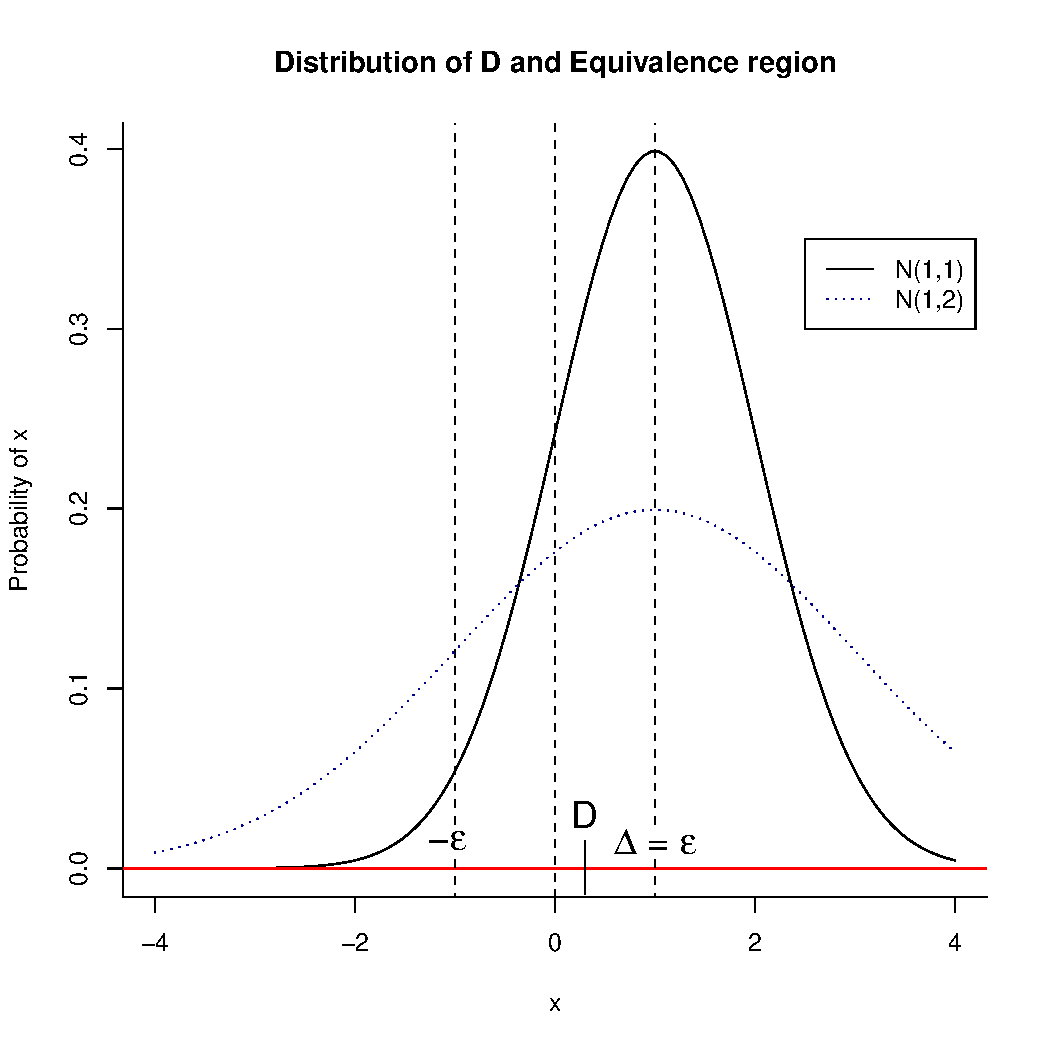
\includegraphics{DiagramNormal.pdf}
\end{center}
\caption{ The solid black line is a plot of the density function of a normal distribution with mean $\mu = \epsilon = 1$ and variance $\sigma = 1$ and the dotted blue line is a plot of the normal distribution  function for $\mu = 1$ and  $\sigma = 2$. The hash mark labelled $D$ is a hypothetical observation of a sample mean. Translating the mean of the distribution in the positive direction necessarily results in a lower likelihood of observing a sample mean inside $(-\epsilon, \epsilon)$. Increasing the standard deviation (and hence its estimator, the standard error), decreases the area beneath the curve between $\pm \epsilon$, decreasing the likelihood of measuring $D$ inside $I_\epsilon$. Finally, with mean $\epsilon$, measurements of sample mean less than $D$ in absolute value are less likely.}
\label{DiagramNormal}
\end{figure}

The distance from $D$ to the nearest endpoint of $I_\epsilon$ in units of standard errors of $D$ is given by 
\begin{eqnarray}
 K = \frac {\epsilon - |D| }{\mbox{SE}(D) },
 \end{eqnarray} 
 where SE$(D)$ is the standard error\footnote{ The standard error is an estimate of the population standard deviation. A common estimate is the sample standard deviation, given by the squared deviations from the sample mean divided by the degrees of freedom. I.e. if  $x = (x_1, \dots x_{n_x})$, then the standard error of $x$ is given by 
 $\sqrt{ \frac{1}{n_x-1} \sum_{i=1}^n (\bar{x} - x_i)^2}$ }
 of the mean difference between the $x$'s and the $y$'s. $K$ not only satisfies the conditions suggested above, but is also a measurement of a $t$-statistic, as described in Appendix \ref{Linear Regression}, meaning we can compare probability of measuring the value $K$ against the probability of  values less likely under the null. Under the null, we would expect intervals larger than $K$ to be less likely. Hence the p-value of the measurement $K$ is given by:
\begin{eqnarray}  
\label{significancelevel}
p &=&  \mathbb{P}( \mathfrak{t} \geq K),
\end{eqnarray}
where $ \mathfrak{t}$ is a Student's $t$ distributed  random variable with $n_x+n_y -2$ degrees of freedom, this probability is easy to calculate.\footnote{ If $\mathfrak{t}$ has $\nu$ degrees of freedom, $\alpha = 1 - \int_{-\infty}^K   \frac{ \Gamma (\frac{\nu+1}{2}) }{\Gamma(\frac{\nu}{2 }) } \frac{1}{\sqrt{\nu \pi}} \left( 1 + \frac{t^2}{\nu} \right) ^{-\frac{\nu+1}{2}} dt $, where $\Gamma(\cdot)$ is the Gamma function. See \cite{Intro} for more detail.}

%The factor of $2$ on the right hand side of equation \ref{significancelevel} comes from the fact that while $D$ is normal, $|D|$ is not. We need to consider both $D$ and $-D$, and hence both the distances 
%\begin{eqnarray} -K &=& \frac{-\epsilon + D}{\mbox{SE}(D) }
 %\\ & \mbox{and}& \\
%K &=& \frac{\epsilon - D}{\mbox{SE}(D) }. \end{eqnarray}
%Hence the p-value is really given by $ \alpha = \mathbb{P}(-K \geq \mathfrak{t} \  or \  \mathfrak{t} \geq K) = \mathbb{P}(-K \geq \mathfrak{t}) + \mathbb{P}( \mathfrak{t} \geq K)  $. Because the Student's $t$ distribution is symmetric about zero, this reduces to $2\cdot  \mathbb{P}( \mathfrak{t} \geq K)$, and hence equation \ref{significancelevel}.  

Rather than the method described above, for computational efficiency, an equivalent formulation of the t-test test, expressed in the language of confidence intervals, is used. We compare the limits of a level $1 - 2 \alpha$ confidence interval symmetric about $D$ to $I_\epsilon$. The level of this confidence interval is $1 - 2 \alpha$ rather than $1 - \alpha$ because it corresponds to the intersection of the rejection regions of two level $\alpha$ one sided tests. Each level $\alpha$ one sided test has a rejection region of area $\alpha$. Hence the complement of their union has area $1- 2 \alpha$. If this interval is contained completely inside $I_\epsilon$, then we have evidence of equivalence at significance level $\alpha$. In other words, we let $n = n_x + n_y -2$ and check if the following condition holds:
\begin{eqnarray} 
\label{conditionconfint}
|D| + t^{1-\alpha}_{n} \cdot \mbox{SE}(D) < \epsilon,
 \end{eqnarray}
where $t^{1-\alpha}_{n}$ is the $(1-\alpha)$-th quantile of the Student's $t$ distribution with $n$ degrees of freedom. If $D$ satisfies this condition, then we have equivalence at level $\alpha$.

A little bit of algebra will show the condition \ref{conditionconfint} is equivalent to \ref{significancelevel}: 
\begin{eqnarray}
|D| + t^{1-\alpha}_{n} \cdot SE(D) < \epsilon \\
\iff \frac{\epsilon - |D|}{\mbox{SE}(D)} > t^{1-\alpha}_{n}
\end{eqnarray}
From the definition of $t^{1-\alpha}_{n}$, if $\mathfrak{t}$ is Student's $t$ distributed with $n$ degrees of freedom,, then we know $t^{1-\alpha}_{n}$ satisfies $\mathbb{P}( \mathfrak{t}  \leq t^{1-\alpha}_{n}) = 1-\alpha$. Hence: 
\begin{eqnarray}
 \mathbb{P}\left(  \mathfrak{t} < \frac{\epsilon - |\Delta_i|}{SE(\Delta_i)} \right) &=& 1 - \alpha, 
 \\ & \mbox{and} & \\
 \mathbb{P}\left(\mathfrak{t} \geq \frac{\epsilon - |\Delta_i|}{SE(\Delta_i)}  \right) &=&  \alpha.
\end{eqnarray} 
which is equation \ref{significancelevel} with $p = \alpha$. The significance level, $\alpha$ of the test, can be thought of as the maximum p-value with which we reject the null. Hence the two formulations of the test are equivalent.






 \section{The Bootstrap Test of Equivalence}
 \label{Bootstrap}
 
 The bootstrap is a non-parametric method\footnote{That is to say: does not rely on the specification of a parametric family prior to statistical analysis.} for ascertaining the accuracy of an estimate, like the t-test. 
 
 \subsection{The Bootstrap Estimate of a Single Parameter}
 For a single parameter, the bootstrap is fairly simple. Suppose we are given  \newline $\mathbb{M} = \nolinebreak ( z_1 , \dots, z_k )$, measurements of a random variable $Z$ from an unknown distribution $F$, and we are interested in some parameter of $F$, called $\theta$, with estimator $\hat{\theta}$. Let the initial calculation of $\hat{\theta}$ be $\hat{\theta}_o$. The bootstrap algorithm is:
 \begin{enumerate}
 
 
 \item Assign probability $\frac{1}{k}$ to each $z_i$, forming the empirical probability distribution $\hat{F}$. 
 
 \item Sample from $\hat{F}$ with replacement $k$ times, obtaining a random sample, $\mathbb{M^*} =  \{z_1^* , \dots, z_k^* \} $. Calculate the same statistic, $\hat{\theta}$, using $\mathbb{M^*}$ as data. 
 
 \item Repeat Step 2  some large number, say $B$, of times, remembering each $\hat{\theta}$ along the way. Call the $i$-th calculation of $\hat{\theta}$ by $\hat{\theta}_i$.
  

 \end{enumerate}
 
This algorithm produces a bootstrapped distribution for the estimator $\hat{\theta}$ which we can use to assess the probability of measuring $\hat{\theta}_o$. Let the bootstrapped estimators be $\Theta = ( \hat{\theta}_1, \dots, \hat{\theta}_B )$. We then specify a critical region based on the bootstrap distribution. We sort $\Theta$ into ascending order. If the significance level of the test is $\alpha$, we select the $(\alpha \cdot B)$$^{th}$ and the $(1 - \alpha) \cdot B$$^{th}$ value, rounding up to the nearest integer when these are not integer values. If these two values lie inside $(-\epsilon, \epsilon)$, then we reject the null.

\subsection{The Bootstrap Test of Equivalence}

In the test of equivalence, rather than a single data set $\mathbb{M}$, our data is divided into two groups, $x$ and $y$, as above. Although the bootstrap works for any statistic which is asymptotically normally distributed, we are explicitly interested in the difference of sample means. Hence, we calculate $\bar{x}$ and $\bar{y}$, and bootstrap the estimates of both means separately. As above, we then resample $n_x$ times from $x$ and  $n_y$ times from $y$. We recompute $\bar{x}$ and $\bar{y}$ from these resamples, and then repeat this process some large number, say $B$, of times. The $i^{th}$ re-computation of $\bar{x}$ is called $\bar{x}^i$, and the $i^{th}$ re-computation of $\bar{y}$ is called $\bar{y}^i$. The bootstrap distribution of the difference: $D =\bar{x} - \bar{y}$ is obtained by considering the differences: $\Theta = ( D_1 = \bar{x}^1 - \bar{y}^1, \dots, D_B = \bar{x}^B - \bar{y}^B )$

The null hypothesis is:
\[ \Delta \notin I_\epsilon \]
In parallel with the t-test test of equivalence above, if $D \notin I_\epsilon$, we cannot reject the null. If $D \in  I_\epsilon$, we ask how likely we are to measure differences as or less likely than $\epsilon$. As we have made no assumptions about the distribution of $D$, we have no reason to suppose any element of $I_\epsilon$ is more likely than any other.  Hence, we simply measure the proportion of the bootstrap distribution which violates the null and compare it to the significance level $\alpha$.  We sort the values of $\Theta$ in ascending order. We call the $\lceil \alpha \cdot B \rceil^{th}$ value $D_{lo}$ and the $ \lceil (1 -  \alpha)\cdot B \rceil$ $^{th}$ value\footnote{The notation $\lceil x \rceil$, where $x$ is a real number, refers to the least integer greater than $x$. } $D_{hi}$. Then, if the interval $(D_{lo}, D_{hi})$ is contained in $I_\epsilon$, we declare equivalence at significance level $\alpha$.  This is exactly the percentile confidence interval described in \cite{BootstrapBook} . 
 


